\documentclass[]{article}       % Default text size and document class

% Format -----------------------------------------------------------------------------
\usepackage[                    % To set up the page
  a4paper,                        % A4 paper
  width=160mm,                    % Text body width
  top=25mm,bottom=25mm,           % Top and bottom margins
  bindingoffset=6mm               % Offset of left and right pages for printing
  ]
  {geometry}
\usepackage{setspace}           % So set spacings (e.g. line height)
  \onehalfspacing                 % Sets line width to 1.5
%\usepackage{sectsty}            % To control sectional headers
%  \chapternumberfont{\huge}       % Set size of chapter number
%  \chaptertitlefont{\huge}        % Set size of chapter title 
\usepackage{multicol}           % Writes in multiple columns
\usepackage{lipsum}             % Inserts blind text for previewing
\usepackage{placeins}           % adding float barriers 
\setlength{\parindent}{0pt}     % remove indentation for new paragraphs

% Language ---------------------------------------------------------------------------
\usepackage[english]{babel}     % To enable language support other than us english
\usepackage[babel]{csquotes}    % Omits spell checking in quotations

% Images, long tables & append pdf pages ---------------------------------------------
\usepackage{float}              % Enables some options for image placement
\usepackage{graphicx}           % To include graphics
\usepackage{                    % Long table stuff
  csvsimple,                      % So a csv can be converted to a table
  longtable,                      % To make long tables
  booktabs                        % To page break long tables properly
  }
\usepackage{pdfpages}           % Appends pdf pages

% Custom fancy image caption ---------------------------------------------------------
\usepackage{caption}
  \captionsetup[figure]{labelsep=space}
%  \captionsetup[table]{labelsep=space}
  \newcommand{\mycaption}[2]{\caption[#1]{\textbar\,\textbf{#1} #2}}

% Math support -----------------------------------------------------------------------
\usepackage{amsmath, amsfonts}  % For fancy math
\usepackage[separate-uncertainty = true, locale=DE]{siunitx} % for SI units
\sisetup{detect-all}

% Citation setup ---------------------------------------------------------------------
\usepackage[]{hyperref}         % To make clickable links
  \hypersetup{hidelinks,}         % To draw no boxes around the links
\usepackage[                    % Citation setup  
    backend=biber,                % Citation backend
    style=authoryear-comp,        % Citation format
    maxnames=1,                   % Max number of names displayed in text
    %sortlocale=de_DE,             % Sorts by german conventions (ß = ss)
    natbib=true,                  % Enables \citep and \citet. Use \parencite and \textcite in future
    url=false,                    % Disaples url
    doi=true,                     % To print the doi
    eprint=false                  % Disables link to eprint (?)
]{biblatex}
\addbibresource{arrenberg.bib} % Where the bibliography file is
\renewcommand{\familydefault}{\sfdefault}
\usepackage{tgheros}
\setlength\bibitemsep{2\itemsep} 

% Abstract title same size as sectional headers --------------------------------------
% see here: https://tex.stackexchange.com/questions/366169/how-to-change-font-size-for-abstract-title
\makeatletter
\renewenvironment{abstract}{%
    \if@twocolumn
      \section*{\abstractname}%
    \else %% <- here I've removed \small
      \begin{center}%
        {\bfseries \Large\abstractname\vspace{\z@}}%  %% <- here I've added \Large
      \end{center}%
      \quotation
    \fi}
    {\if@twocolumn\else\endquotation\fi}
\makeatother


% Document ---------------------------------------------------------------------------
\begin{document}
\begin{titlepage}
\begin{center}

% Head block
\vspace*{0.5cm}
\Large
Protokoll\\
Neurobiologisches Großpraktikum\\
\vspace{1cm}

% Title and author
\Huge
\textbf{Color-blindness of direction-selective units in the zebrafish optic tectum}\\
\Large
\vspace{1cm}
\textbf{Alexander Wendt, Patrick Weygoldt}
\vspace{1cm}

%Add a nice figure below the authors
% \begin{figure}[ht]
%     \centering
%     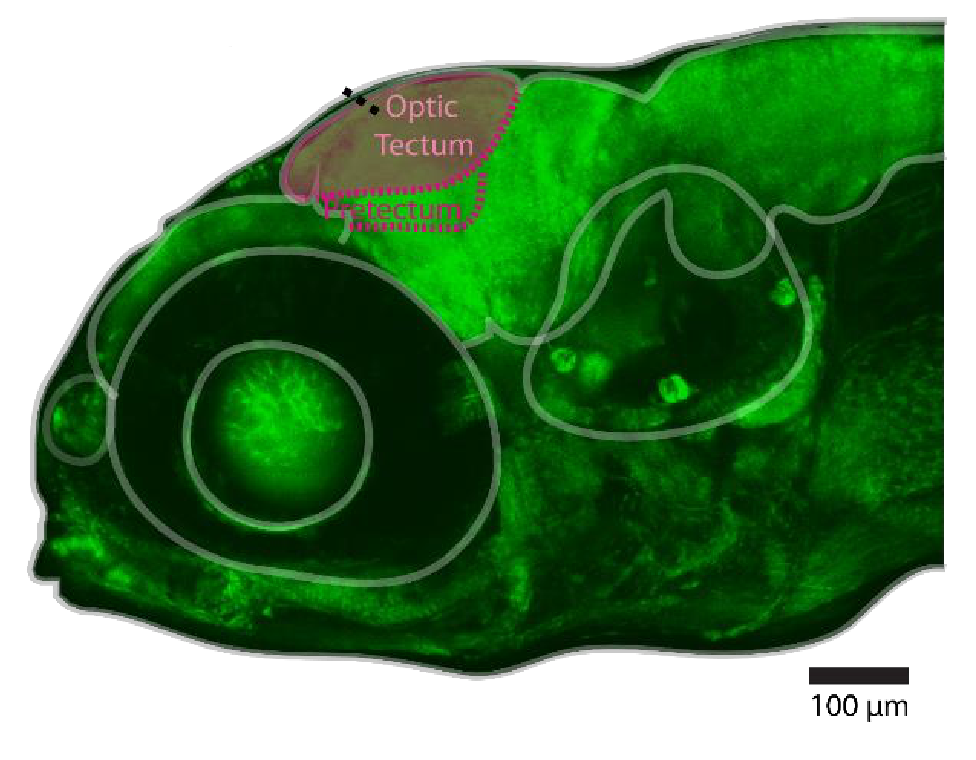
\includegraphics[scale=0.6]{figures/titlepic.png}
%     \mycaption{THIS is NOT A FISH}{Done by the weakly electric fish community}
% \end{figure}
\vfill

% Bottom block
\large
\vspace{0.5cm}
Supervised by:\\
\vspace{0.5cm}
Tim Hladnik, David Burkardt, Aristides Arrenberg\\
Systems Neurobiology\\
Werner Reichardt Centre for
Integrative Neuroscience \\
Tuebingen University\\
\vspace{1cm}
\today \\
\vspace{0.5cm}

        
\end{center}
\end{titlepage}
 % Add the path to the titlepage here

\section{Introduction}
   \label{chap:introduction}
   
Sensory information about our environment is crucial for our survival. Especially the sensory modality of light is essential to perceive the outside world. In primates, for example, the incoming light is perceived by three photoreceptors, and they process the chromatic information \parencite{robert1977retinalcones}. This chromatic information is letting us see the world in color. Another factor processed by the same sensory modality is temporal changes e.g the movement of an object. These two factors, color vision and movement, were thought to be functionally independent of each other. \cite{margaret1988segregationcolormovement} explained this segregation of color and movement by the pathway selectivity and differences in the encoding of \glqq color selectivity, contrast sensitivity, temporal properties and spatial resolution\grqq{} \parencite{margaret1988segregationcolormovement} of cells in the geniculate. For example, cells that encode for color are in a separate pathway (parvocellular geniculate pathway, motion in magnocellular geniculate pathway) and have properties that ensure only color vision \parencite{margaret1988segregationcolormovement}. This separation of pathways from color and motion should then indicate that motion vision is color blind \parencite{MULLEN1992colormotion}. In contrast to Livingstone, \cite{MULLEN1992colormotion} did find a connection between color and motion whereas the motion pathway has some reduced color vision and vice versa, using an isoluminant chromatic test. Further experiments with fMRI in humans also imply that color vision is widely distributed, and not defined for only one pathway \parencite{WANDELL1999fmricolor}. This system which is integrating motion sensitivity can be further subdivided into three orders of processes \parencite{zhong1999isoluminant}. The first-order is responsible for computing movements of objects that are defined by their luminance, whereas the second-order motion detection is defined by the luminance contrast and lastly the third-order motion is defined as figure relative to the background \parencite{zhong1999isoluminant}. \cite{zhong1999isoluminant} displayed that isoluminant motion is computed by the third-order system, which concludes this stimulus is computed in a brain region where \glqq binocular inputs of form, color, depth, motion, and texture are all available \grqq{} \parencite{zhong1999isoluminant}. 

\vspace{\baselineskip}

To summarize this, we tried to emphasize both viewpoints in primates. The first one is separating color and motion in two different pathways whereas the other displays a connection between the color and motion pathway. From an evolutionary perspective, color vision in primates is a recent development \parencite{yokoyama2001colorvisongen} and has influenced to some degree the motion perception in primates. To investigate the evolutionary changes in color-motion perception, we wanted to explore the perception of the zebrafish (\textit{Danio rerio}), compared to primates a very early vertebrate. In fish, the color vision evolved independently from primates, providing a comparative approach \parencite{nigel1967fishretina}. 

\subsection{Motion perception in zebrafish}

Zebrafish as model organisms presents the unique opportunity to combine whole-brain imaging data with behavior to complex visual stimuli \parencite{bollmannZebrafishVisualSystem2019}. The retina of the zebrafish has a similar cell structure and pathways compared to mammalian retinas, which makes the comparison easier \parencite{bollmannZebrafishVisualSystem2019}. The visual system is developed early after fertilization, in a time span of three days \parencite{stuermer1988retinotopic}, but after the three days, zebrafish reliably respond to light \parencite{zhang2010development}. If one would fixate on the body (leaving the eyes movable) and stimulate the fish with a whole-field motion, then it would elicit an optokinetic response (OKR). OKR describes then the movement of the eyes in the direction of the stimulus \parencite{brockerhoff1995behavioral}. This OKR is encoded in the velocity-to-position neural integrator (VPNI) which is located in the caudal hindbrain \parencite{miri2011regression, miri2011spatial}. Aside from this circuitry for the OKR, \cite{perez2016sustained} results indicate that direction-selective tectal cells had a sustained rhythmic activity after stimulation. \cite{wangParallelChannelsMotion2020} investigated receptive fields of the pretectum and tectum of motion-selective neurons. Neurons in the pretectum have large receptive fields for the lower visual fields, whereas tectal neurons have mostly small receptive fields for the upper nasal visual field \parencite{wangParallelChannelsMotion2020}. This underlines the notion that motion-selective cells in the pretectum and tectum correspond to different functions. The pretectum is important for the optomotor response (OMR), where fish swim in the direction of the optic flow, and the tectum for near-field prey capture \parencite{wangParallelChannelsMotion2020}. 

\subsection{Color vision in zebrafish}

Color vision, on the other hand, is first perceived in the four photoreceptors with absorption peaks around \SI{500}{\nano\meter} (red), \SI{470}{\nano\meter} (green), \SI{410}{\nano\meter} (blue), and \SI{360}{\nano\meter} (UV) \parencite{robinson1993zebrafish}. The photoreceptors are arranged in a pattern which is called \glqq cone mosaics\grqq{}, and the ratios between photoreceptors in larval to adult zebrafish change \parencite{allison2010ontogeny}. The proportions of the photoreceptors change in the development but the position of the receptors is evolved to fit for the natural stimuli, above the fish, in  a natural scenery are hardly any color. Therefore the retina encoding for light trajectories coming from above the fish is primarily achromatic \parencite{zimmermannZebrafishDifferentiallyProcess2018}. More color is found beneath the fish and the horizontal level, which is represented in the retina \parencite{zimmermannZebrafishDifferentiallyProcess2018}. After the retina visual stimuli are processed by the optic tectum, if compared to a mammalian structure, is homologous to the superior colliculus, and also the pretectum and thalamus \parencite{bollmannZebrafishVisualSystem2019}. 

\subsection{Aim of this work}
The first seperation of color and motion in zebrafish was shown behaviorally by \cite{orgerChannelingRedGreen2005}. They could show that zebrafish larvae are motion blind to a chromatic (isoluminant) stimulus, using a motion nulling method \parencite{chichilniskyFunctionalSegregationColor1993}. The physiological segregation of color and motion in the zebrafish brain is still unclear.  We investigated this question with a new setup, that can stimulate the fish globally with color gratings and simultaneously record  CA imaging data of the optic tectum and pretectum with a 2-photon infrared laser. 


% \begin{itemize}

% \item Early on, photoreceptors
% sort by wavelength (Marks et al., 1964; Marc \&  Sperling, 1977),
% while bipolar cells sort increments and decrements of light (Werblin \& Dowling, 1969).
% \href{https://www.cambridge.org/core/journals/visual-neuroscience/article/channeling-of-red-and-green-cone-inputs-to-the-zebrafish-optomotor-response/180B0E41BDD8D237586D42D07B9908E0}{oger2005}

% \item Stimulus color and contrast influence perceived stimulus speed. For example, a stimulus can be made to appear to move at a different rate by adjusting its color or contrast (Cavanagh et al. 1984). \href{https://doi.org/10.1016/S0896-6273(00)81037-5}{wandall1999}

% \item "in vision, specializations are often
% made according to the statistics of specific regions in visual
% space. For example, mouse cones preferentially process dark
% contrasts above, but not below, the visual horizon, likely boosting the detection of aerial predators [3, 4]."  
% \href{https://doi.org/10.1016/j.cub.2018.04.075}{wangarrenberg2020motion-extraction}



% \item \textbf{Vision in zebrafish}
% \item Zebrafish larvae perform a wide range of visually mediated behaviours, ranging from prey capture
% (Trivedi and Bollmann, 2013; Mearns et al., 2020) and escape behaviour (Heap et al., 2018) to stabilisation behaviour (Kubo et al., 2014; Orger et al., 2008); however, the importance of stimulus
% location within the visual field for the execution of the respective behaviors has only recently been
% recognized and is still not well understood (Hoy et al., 2016; Zimmermann et al., 2018;
% Mearns et al., 2020; Kist and Portugues, 2019; Wang et al., 2020; Johnson et al., 2020;
% Lagogiannis et al., 2020)
% \href{https://doi.org/10.7554/eLife.63355}{Dhemelt2021stimulus-location}

% \item Within three days of hatching, larval zebrafish become highly
% visual animals with tetrachromatic wide-angle vision [9, 10] and
% well-studied visual behaviors [11–16]. 
% \href{https://doi.org/10.1016/j.cub.2018.04.075}{wangarrenberg2020}

% \item the two eyes make up nearly a quarter
% of the total body volume, with the neuronal retina taking up $>$75\%
% of each eye. Indeed, about half of the larva’s central neurons are
% located inside the eyes (STAR Methods). 
% \href{https://doi.org/10.1016/j.cub.2018.04.075}{wangarrenberg2020}

% \item \textbf{our experiment}
% \item motion-nulling method \href{https://doi.org/10.1016/0042-6989(93)90010-T}{chichilnisky1993motion-nulling}
% \end{itemize}

\pagebreak
\section{Methods}
  \label{chap:methods}
  \subsection{Experimental animals}

We used three transgenetic zebrafish from Janelia farm with a good expression of Gcamp6 gen ($tg(HuC:GCamp6f)jf7$). For the experiments, the zebrafish were 5-6 days postfertilization (dpf) old. In two of the three, we recorded behavioral data.    

\subsection{Experimental setup}

The stimulation arena consisted of a glass bulb that was coated in paint to be able to project light on it from the outside. The light was produced by a high power LED light source (CHROLIS-C1, Thorlabs Incorporated) and transmitted to a projector (DLP® LightCrafter™ 4500, Texas Instruments Incorporated) using a liquid light guide. The light exiting the projector was then reflected downwards in a \SI{90}{\degree} angle onto a square pyramidal mirror, that split the beam into four. Each of the four beams was then reflected by one of the four mirrors placed around the setup and consequently projected onto the glass sphere. The result is a spherical projection. The experimental setup is visualized in figure \ref{fig:setup}. The fish were embedded in Agarose on a custom designed stage that could be fixed inside the stimulus arena.  

\begin{figure}[H]
    \centering
    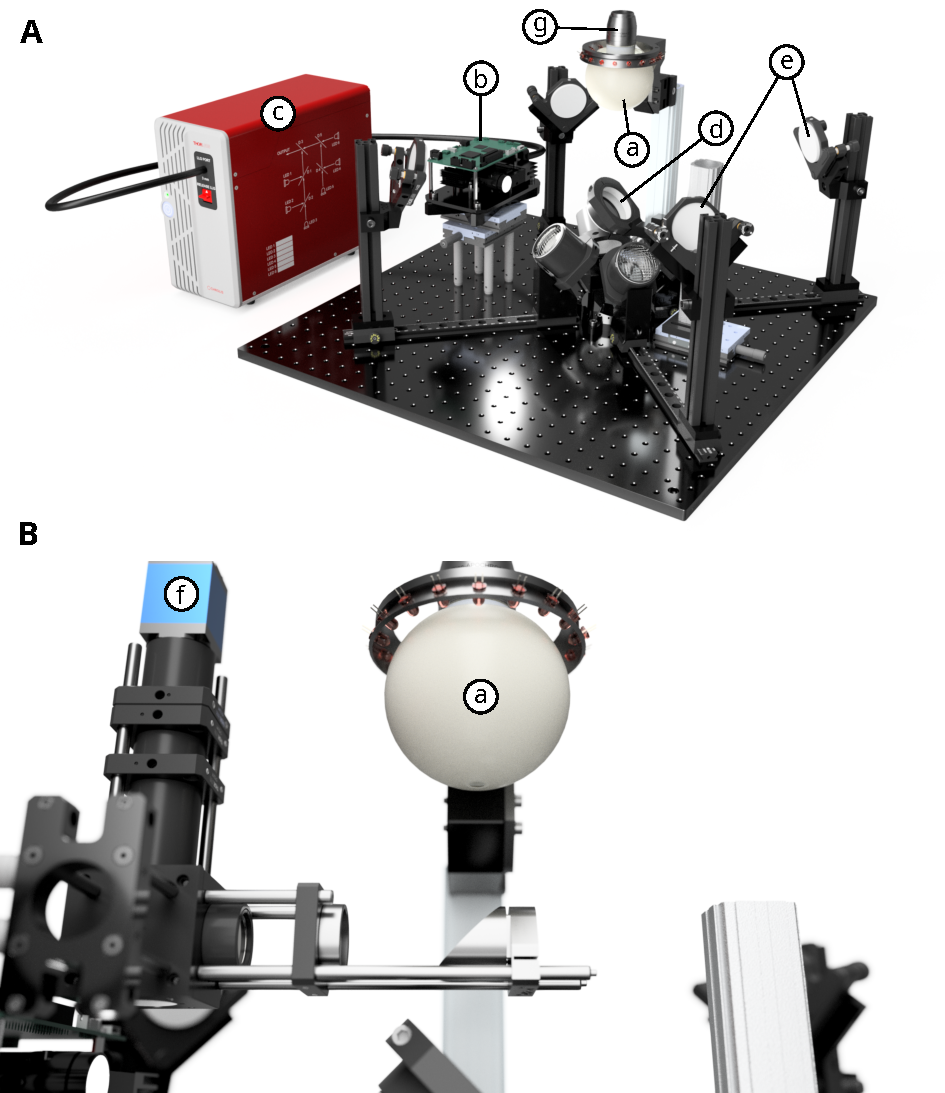
\includegraphics[width=0.6\textwidth]{figures/setup.pdf}
    \mycaption{CAD rendering of the experimental setup.}{\textbf{A} shows the whole recording setup excluding the camera recording behaviors of the fish. The fish is fixed inside a glass bulb (a) containing E3 medium. The light is produced by an LED light source (c), transferred to a projector (b) and projected onto a \SI{45}{\degree} mirror (d). The mirror reflects the projection onto a pyramid mirror (not visible in the current rendering), which splits the beam into four. The four beams are then reflected by four mirrors placed around the setup (e) and reflected onto the glass bulb from four sides. The result is a spherical projection into the glass bulb.The calcium activity was recorded by a moving objective microscope that peeks through an opening in the top of the glass sphere (g). \textbf{B} shows the camera (f) used to record through the bottom of the glass bulb using mirrors as well. Images are courtesy of Tim Hladnik.}
    \label{fig:setup}
\end{figure}

\subsubsection{Embedding procedure}

\begin{wrapfigure}{R}{0.5\textwidth}
    \vspace{-0.3cm}
    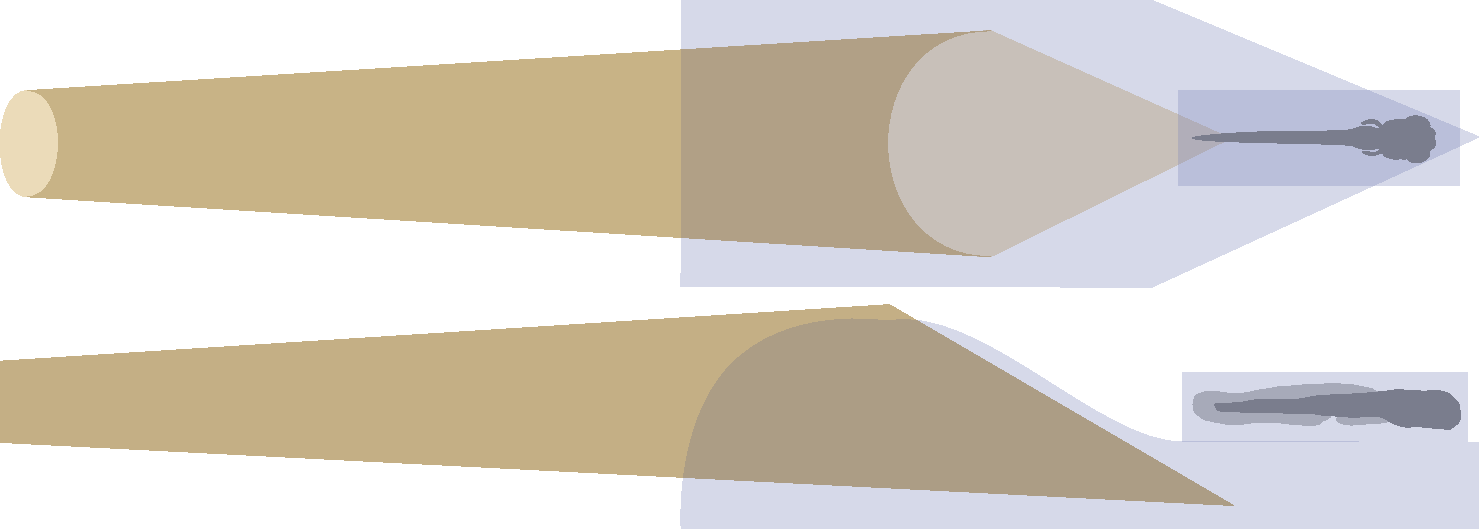
\includegraphics[width=\linewidth]{figures/drawing.pdf}
    \mycaption{Agarose stage}{ to fixate the larvae. The stage consisted of a diagonal cut-off of a pipette tip (orange) and a small, pointed Agarose table (blue). The fish (gray) were separately embedded into a drop of Agarose. We pruned the edges and then placed the Agarose block containing the fish onto the point of the Agarose table.}
    \label{fig:stage}
\end{wrapfigure}

The immobilization of the fish was conducted with \SI{1.6}{\percent} low-melting Agarose, where it was submerged for a short time before a drop of Agarose containing the fish was placed on a Petri-dish to polymerize. Meanwhile, the plastic pipette was prepared (diagonal cut-off, see figure \ref{fig:stage}), placed on a 3D-printed stage, and filled with \SI{2}{\percent} Agarose. After \SI{30}{\minute} the stage was separated from the now polymerized Agarose. The immobilized fish was placed on the tip of the Agarose that stood out from the pipette tip. To combine the Agarose from the pipette and the Agarose where the fish was in, we added \SI{1.6}{\percent} Agarose which filled the gap between those two Agarose blocks. The pipette was then inserted into a holding apparatus inside the glass sphere, which we filled with E3. For two of the three fish, we removed the Agarose around the eyes of the fish, so that the fish can move them (Figure \ref{fig:stage}). 

\subsubsection{Stimulus}

The stimulus consisted of red and green gratings with six different logarithmically increasing contrast levels (0., 0.1, 0.18, 0.32, 0.56, 1.0) that were randomized. The stimulus time for one contrast level was 8 seconds long, divided into 4 seconds of no angular velocity and followed by 4 seconds with an angular velocity of \SI{30}{\degree\per\second}. Two directions of velocity were used and they were randomized. This protocol was repeated 3 times and the order stayed the same across the repeats. Before the protocol started and after the protocol ended we implemented a pause with no stimulus for 15 seconds. The stimulus was generated using \href{https://github.com/thladnik/vxPy}{vxPY} (\href{https://github.com/thladnik/vxPy}{https://github.com/thladnik/vxPy}). The color contrast levels of the stimulus we displayed for this experiment were not yet linearised and which contrast levels the fish exactly perceived are unknown. 

\subsubsection{Calcium imaging}

Calcium imaging was conducted with an infrared laser (Coherent Vision-S Ti-Sa laser, and a 25 x objective (Nikon CFI75, Tokyo, Japan),  a wavelength of \SI{920}{\nano\meter}), with a movable objective microscope (MOM) (Sutter Instruments, Novato, CA, USA). The resolution of the calcium imaging was \SI{2}{\hertz}. Before beginning the imaging protocol we checked if the fish was drifting out of the focal plane. For this procedure, we took a reference image and waited for \SI{30}{\minute}, after that time we retook the image, compared it with our reference image and decided to start our stimulus protocol or to wait another \SI{30}{\minute}. Calcium imaging was done in \SI{10}{\micro\meter} intervals along the optical axis. After each recording, we visually assessed the drift of the Agarose. If drifting occurred, we did not consider these recordings for the data analysis. For our three fish, we used 12, 5, and 5 recordings. For processing the Calcium-imaging data, we used suite2p, an open-source pipeline for processing two-photon calcium imaging data \parencite{Pachitariu061507}.

\subsubsection{Behavioral response}

For a behavioral measure of the sensitivity to isoluminant chromatic motion stimuli, we chose the optokinetic response (OKR). 
Eye movements were recorded via a camera that recorded the bottom of the larva through a \SI{45}{\degree} mirror below the glass bulb (see figure \ref{fig:setup}). A small area on the bottom of the bulb was not coated in paint and thus enabled a clear view into the underside of the fish. Image segmentation and eye tracking happened in real-time using \href{https://github.com/thladnik/vxPy}{vxPY} (\href{https://github.com/thladnik/vxPy}{https://github.com/thladnik/vxPy}). Eye velocities were recorded in degrees per second at a rate of \SI{20}{\hertz}.  

\subsection{Data analysis}

We wrote our data analysis pipeline in Python 3.10.9 using the packages Numpy \parencite{harris2020array}, Scipy \parencite{2020SciPy-NMeth}, Matplotlib \parencite{Hunter:2007}, vxPy (\href{https://github.com/thladnik/vxPy}{https://github.com/thladnik/vxPy}) and suite2p \parencite{Pachitariu061507}. All scrips used for the analysis and plotting are publically available in a \href{https://github.com/weygoldt/colorblind-directioncells}{git repository}.

\subsubsection{Calcium data}

First, we computed the $\operatorname{dff}$ of the fluorescence signal of every single ROI by formula \ref{eq:dff}.

\begin{equation}
    \operatorname{dff}(t) = \frac{f_{ROI}(t) - \langle f_{ROI}(t) \rangle}{\langle f_{ROI}(t) \rangle}
    \label{eq:dff}
\end{equation}

Where the difference between the fluorescence of a single point in time $f_{ROI}(t)$ and the mean of the signal over time is divided by the mean. We further used the $\operatorname{dff}$ to compute the Z-score to quantify calcium activity (equation \ref{eq:zscore}).

\begin{equation}
    Z = \frac{\operatorname{dff}(t) - \langle \operatorname{dff}(t) \rangle}{\sigma_{\operatorname{dff}(t)}}
    \label{eq:zscore}
\end{equation}

The Z-score indicates how many standard deviations a certain point in time deviates from the mean of the signal, in this case, the $\operatorname{dff}$ of the signal. This is particularly useful in this context because peaks that originate from noise (in signals with a large standard deviation) are scaled down relative to peaks with a good signal-to-noise ratio. To simplify the analysis of multiple time series with different sampling rates, we computed for every separate stimulation phase the mean of the z-score and dff. This was possible because the sampling rate of the microscope was relatively low (\SI{2}{\hertz}) and the stimulation phases were short. Taking the means significantly simplified the analysis while resulting in a minor loss of temporal resolution.

\vspace{\baselineskip}

\begin{figure}[ht]
    \centering
    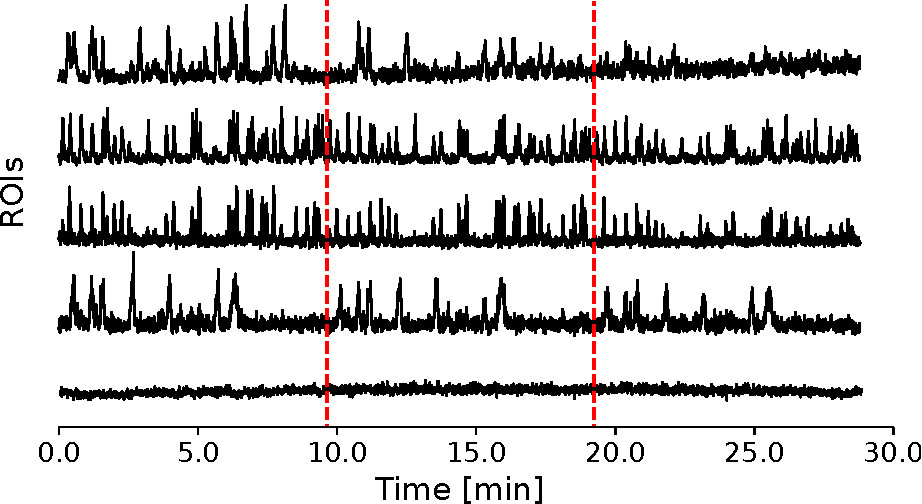
\includegraphics[width=0.8\linewidth]{figures/autocorrelation.pdf}
    \mycaption{Calcium signal (Z-score) over time }{ from various ROIs. Red lines indicate the three repetitions.}
    \label{fig:autocorrelation}
\end{figure}

Since we targeted specifically direction selective cells, we constructed a data filtering pipeline that only provides the ROIs that respond to movements in a certain direction. In a first filtering step we excluded all individuals that did not respond to the stimulus. To do so, we computed the Spearman correlations between the z-scores of the same ROI across the three identical repeats of the stimulation. This resulted in three correlation coefficients per ROI, from which we then took the mean. To choose the units with the strongest auto-correlation, we estimated the distribution of the resulting correlation coefficients by a convolution with a Gaussian kernel. We then chose the ROIs that fell into a 20\% integral of the right tail of the distribution (Figure \ref{fig:autocorrelation}).

\begin{figure}[H]
    \centering
    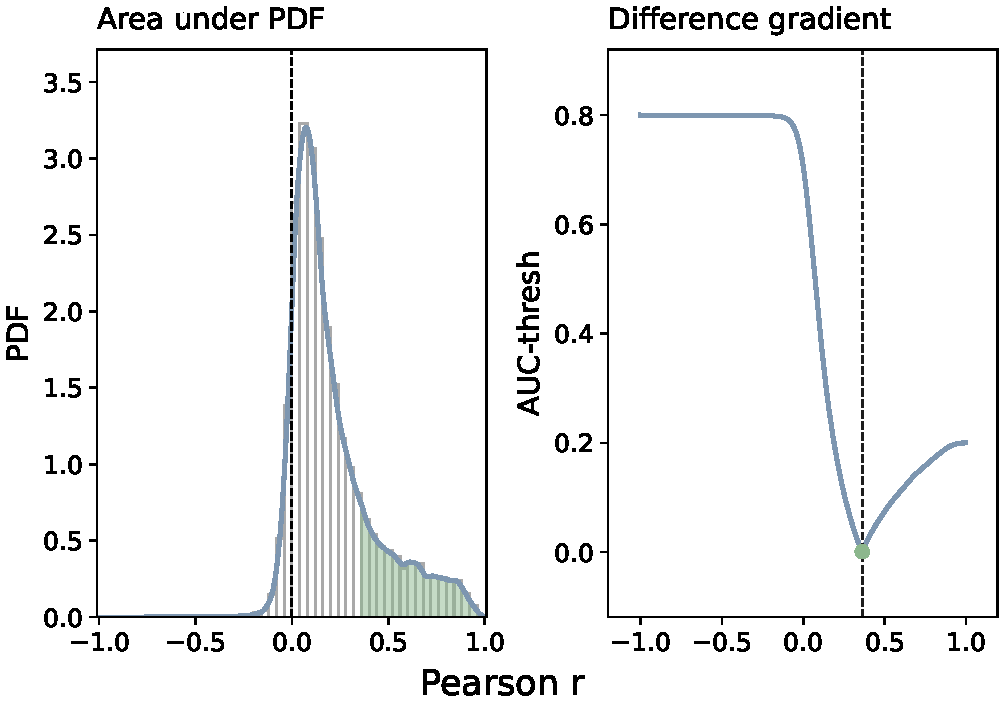
\includegraphics[width=0.8\linewidth]{figures/pcorrelation.pdf}
    \mycaption{Probability density of autocorrelations.}{ \textbf{Left:} Probability density function of the mean correlation coefficients computed between the stimulation repeats of a single ROI. The green tail indicates the area that was chosen to include the 'active' ROIs, i.e. the ones that were correlated strongly between the trials, which indicates repeatable response to the stimulus. \textbf{Right: }Difference gradient that was used to obtain all ROIs that fall into the green area. To obtain this, we computed the area under the curve (AUC) between the one and an array of index values and then subtracted it from our target AUC of 0.2.}
    \label{fig:pcorrelation}
\end{figure}

In a next filtering step, we had to select all ROIs that responded specifically to either clockwise or counterclockwise motion. To do so, we created motion regressors for either direction and correlated them with the z-scores. All ROIs that crossed the correlation threshold of 0.2 were included in the analysis. Figure \ref{fig:regressor} shows an example of some z-scores and the regressors. In a next step, we removed all stimulus phases where no motion stimulus was presented and then computed the means and standard deviations for each stimulus categories for all fish and all repeats for a single fish. 

\begin{figure}[H]
    \centering
    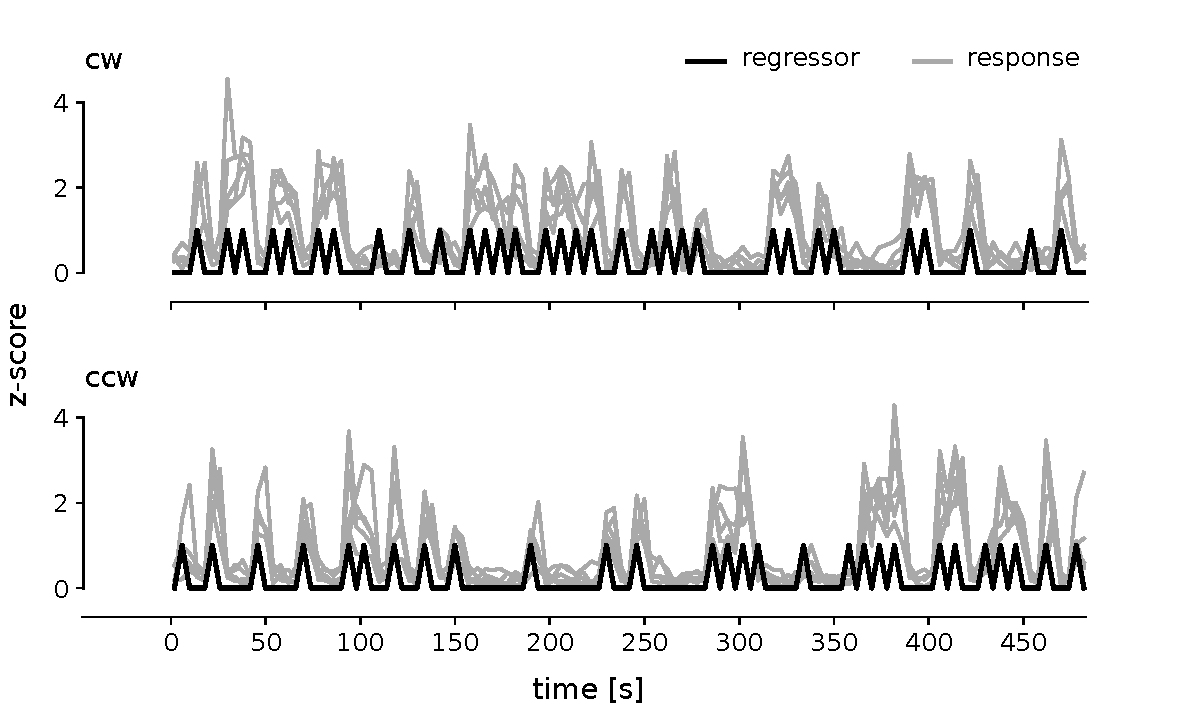
\includegraphics[width=0.8\linewidth]{figures/regressor.pdf}
    \mycaption{Motion-direction regressors and correlated z-scores. }{The black line show the regressors for clockwise (cw, top) and counterclockwise (ccw, bottom) respectively. The gray lines indicate the z-scores of some ROIs that were strongly correlated with the respective regressors.}
    \label{fig:regressor}
\end{figure}

\subsubsection{Behavioral data}

As a behavioral measure we chose the eye velocities. To make the velocities comparable across the stimulus categories we removed saccades in the signal by a median filter with a width of 41 data points. As in the calcium signal, we then computed the mean eye velocity for each stimulus phase. The second step of abstraction was to compute the means and standard deviations across stimulus repeats and across the two individuals we recorded behavioral data for.  

\FloatBarrier

\pagebreak
\section{Results}
  \label{chap:results}
  \subsection{Direction selective units in the optic tectum}

In total, we recorded 14371 units in the optic tectum of 3 zebrafish larvae (Figure \ref{fig:heatmap}). Our preprocessing pipeline extracted 129 units to be distinctly direction selective for either ccw or cw movement. Figure \ref{fig:heatmap} serves as an overview of the data set after it passed our preprocessing pipeline. The shade of the heatmap encodes the z-score of the respective ROI in the respective stimulus phase. It also illustrates the raw data, i.e. in the recorded temporal resolution instead of the means per phase. The bar on top illustrates single stimulus phases by a green and a red bar. The constrast levels for green and red where linearized for visualization purposes. Data in figure \ref{fig:heatmap} is visualized excluding the pauses of stimulation. Additionally, the previously randomized stimulation phases (motion direction and contrast levels) are now sorted. The left side shows the ccw moving stimulus phases and the right side the cw moving phases. On each side, all levels of green contrast are sorted by their combination with red contrast. The lowest row of the heatmap includes a subset of the units we excluded from our analysis. The second line from the bottom illustrates a subset of units that were considered to be 'active', i.e. showed auto-correlations that crossed our threshold. The two rows above show the complete dataset that passed the filtering steps and was included in the analysis. These rows nicely illustrate that the direction selective units we picked from the dataset using the regressor-correlation only show activity for their respective rotation direction. If we consider the chromatic stimulus levels, the same pattern appears in both populations: For stimuli with strong achromatic contrast, i.e. where red contrast is zero and green contrast increases (left sides of ccw and cw colums), the recorded calcium activity increases with increasing luminance contrast. If we consider the right side of the stimulus column for both populations, i.e. where red contrast is strongest and green contrast increases, we see the opposite pattern: While the luminance contrast is high, calcium activity is strong. But as the stimulus approaches isoluminance, i.e. chromatic contrast becomes the main driver of the response, calcium activity decreases.

\vspace{\baselineskip}

\begin{figure}[ht]
    \centering
    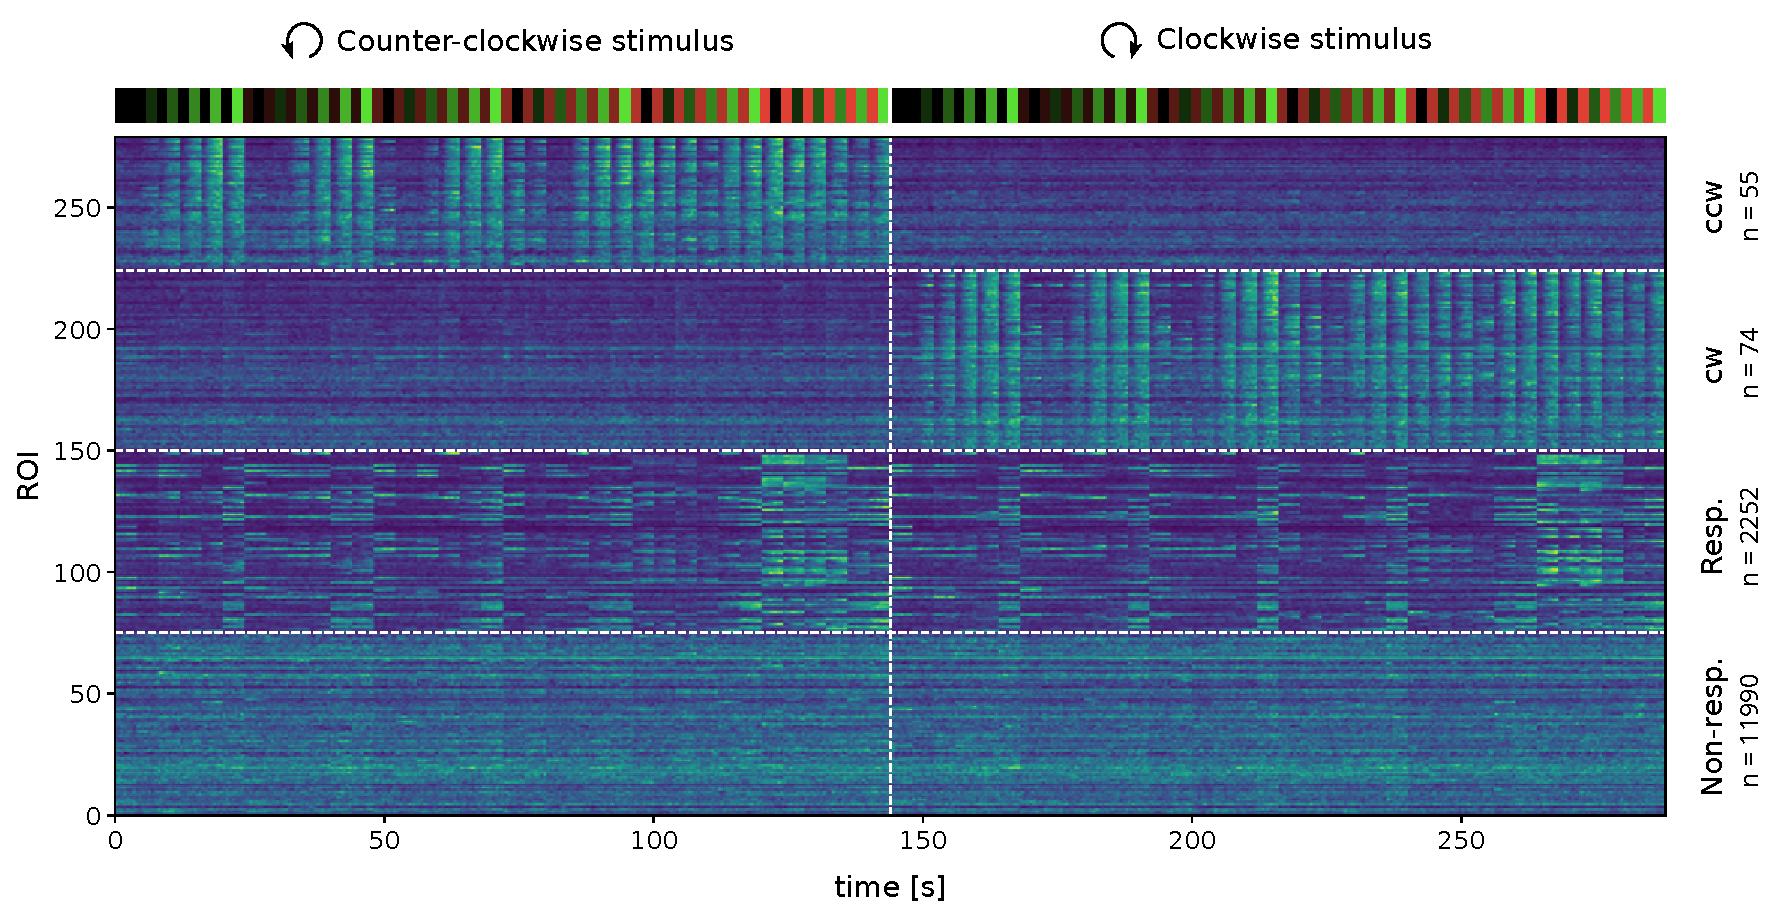
\includegraphics[width=\linewidth]{figures/testimg.pdf}
    \mycaption{Overview of selected ROIs}{ after they passed through our preprocessing pipeline. As opposed to our stimulus protocol, the data is sorted according to rotation direction and contrast levels. Data is plotted for just the fist of three stimulus repetitions. Units in the lowest category show now apparent pattern of activity in response to the stimulus. Units that are considered to be just responsive but not direction selective show a pattern that corresponds to the stimulus but does not change between the two rotation directions. Unit that where selected to be direction selective only show an activity pattern that corresponds to the stimulus in their respective rotation direction.}
    \label{fig:heatmap}
\end{figure}

In figure \ref{fig:calciumdata} we only included direction selective units and computed the mean and standard deviations for every stimulus phase across all individuals, ROIs, and repeats. The resulting data is plotted as a line plot for the combination of every single possible level of green contrast separately combined with all possible combinations of red contrast (figure \ref{fig:calciumdata}, (B) ). This is the same order that we chose to visualize the stimulus in figure \ref{fig:heatmap}. If the units we recorded did not respond to isoluminant chromatic contrasts, the line plots should show a trough where the red and green contrast is the same. This point is denoted by a dashed vertical line. For a green contrast level of 0 the minimum for both cw and ccw line plots is at 0. This is to be expected since motion is not supposed to be encodable if there is neither luminance nor chromatic cues that make it perceivable. For the green contrast levels of 0.1 and 0.18 however, the minima are both just right of the dashed vertical line. This indicates firstly, that a isoluminant chromatic contrast evokes the lowest response in direction selective units and secondly, that the green channel was perceived stronger than the red channel by the fish. The same pattern is observable for a green contrast of 0.32. For green contrast levels above that no trough is visible. 

\vspace{\baselineskip}

In figure \ref{fig:calciumdata}, (C) top, we visualized all possible stimulus combinations in the same way we visualized the mean z-scores from (B): All possible levels of green are plotted in the columns of the matrix and all possible levels of red contrast are plotted in the rows of the matrix. The luminance contrast increases strongest along the x- and y-dimension of the matrix, while the isoluminant, chromatic contrast increases along the diagonal of the matrix. Below that we then visualized the average z-scores that are already plotted in (B) in the same way. The resulting heat map shows an increase in the z-scores along the x- and y-axes, i.e. where luminance contrast increases. The diagonal, where the stimulus was assumed to be isoluminant and consisting of exclusively chromatic contrast, the heat map has a local minimum. This shows, that stimuli with more chromatic contrast than luminance contrasts resulted in lower activity in the direction selective neurons of the optic tectum. In addition, the heat map shows stronger activation along the x-axis (green contrast increase) compared to the y-axis (red contrast increase). This, in combination with the notion that the diagonal of inactivity is shifted towards the red channel, supports the assumption that the green channel was perceived stronger by the fish.


\begin{figure}[ht]
    \centering
    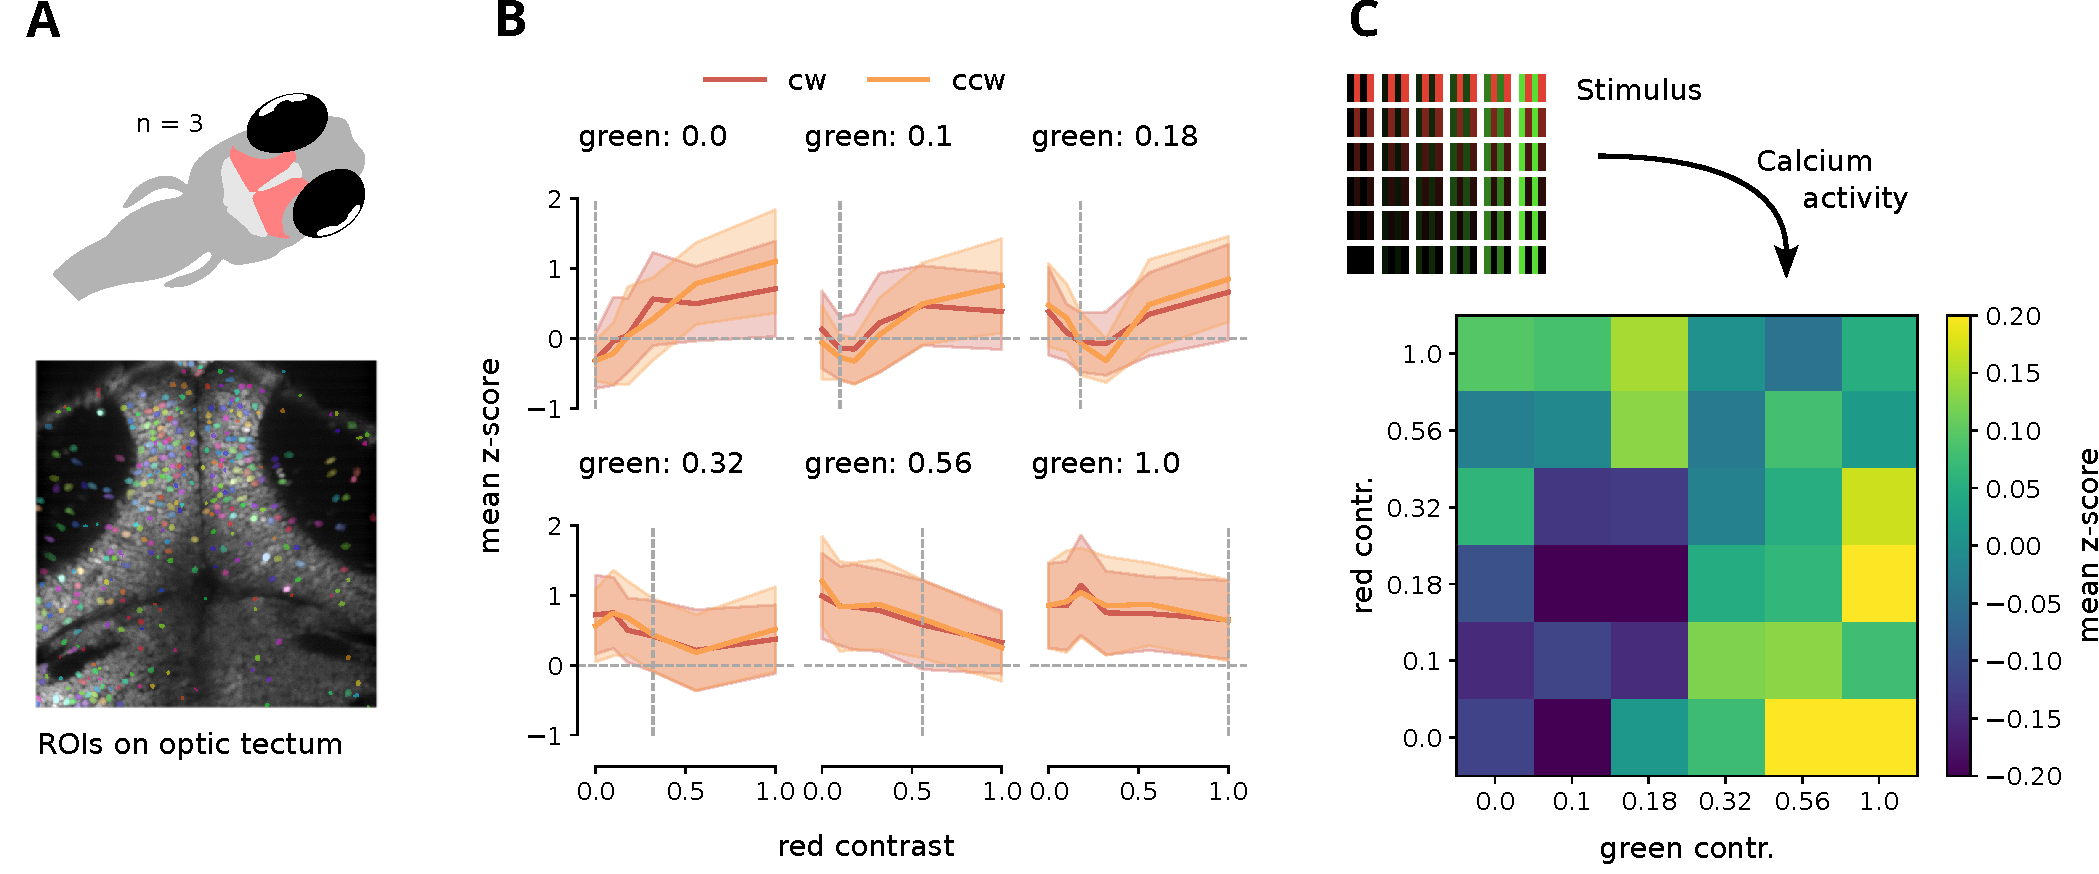
\includegraphics[width=\linewidth]{figures/contrast_curves_ca.pdf}
    \mycaption{Calcium activity for different contrast levels.}{(A) Location of the optic tectum in the brain of a zebrafish embryo. The lower figure illustrates the regions of interest in the optic tectum for which the activity was measured. (B) The mean z-score in all active units for ccw (orange) and cw (red) direction selective units. Each subplot shows the mean and standard deviation for one distinct level of green contrast in comparison to all possible combination of red contrast for this respective green level. The dashed vertical line denotes the value on the x-axis for which only color contrast was expected to drive a response. Thus we expect troughs in activity at the positions of the dashed line. (C) Shows the different levels of the stimulus contrast illustrated in a matrix where red contrast decreases in each row and green contrast increases in each column. The heat map below illustrates the mean z-score pooled for both rotation directions organized in the same way as the stimulus matrix. If given the assumption that red and green contrast was perceived equally and that color contrast alone does not drive the activity of motion direction selective units, we expected diagonal with low z-scores.}
    \label{fig:calciumdata}
\end{figure}

\subsection{Optokinetic response}

Figure \ref{fig:behavdata} shows the recorded eye velocities in a similar manner as the calcium data visualized in figure \ref{fig:calciumdata}. Panel (B) shows the mean eye velocities in all stimulus phases computed across both subjects and all stimulus repeats. Each subplot illustrates a single level of green contrast in combination with all possible levels of red contrast. If the driver of the observed behavior was luminance more than chromaticity, we should again see a trough in the mean eye velocity where the levels of green and red contrasts were the same, i.e. at the dashed vertical lines. As in figure \ref{fig:calciumdata}, the trough approximately follows the dashed vertical line through the subplots. Again, the same pattern is observable in panel C of figure \ref{fig:behavdata}. The diagonal includes the lowest mean eye velocities, suggesting that the behavioral response was mainly driven by the luminance, instead of chromaticity. As in figure \ref{fig:calciumdata} (C), the diagonal is slightly shifted upwards. This further strengthens our assumption, that the green channel was perceived with a higher intensity. 

\begin{figure}[H]
    \centering
    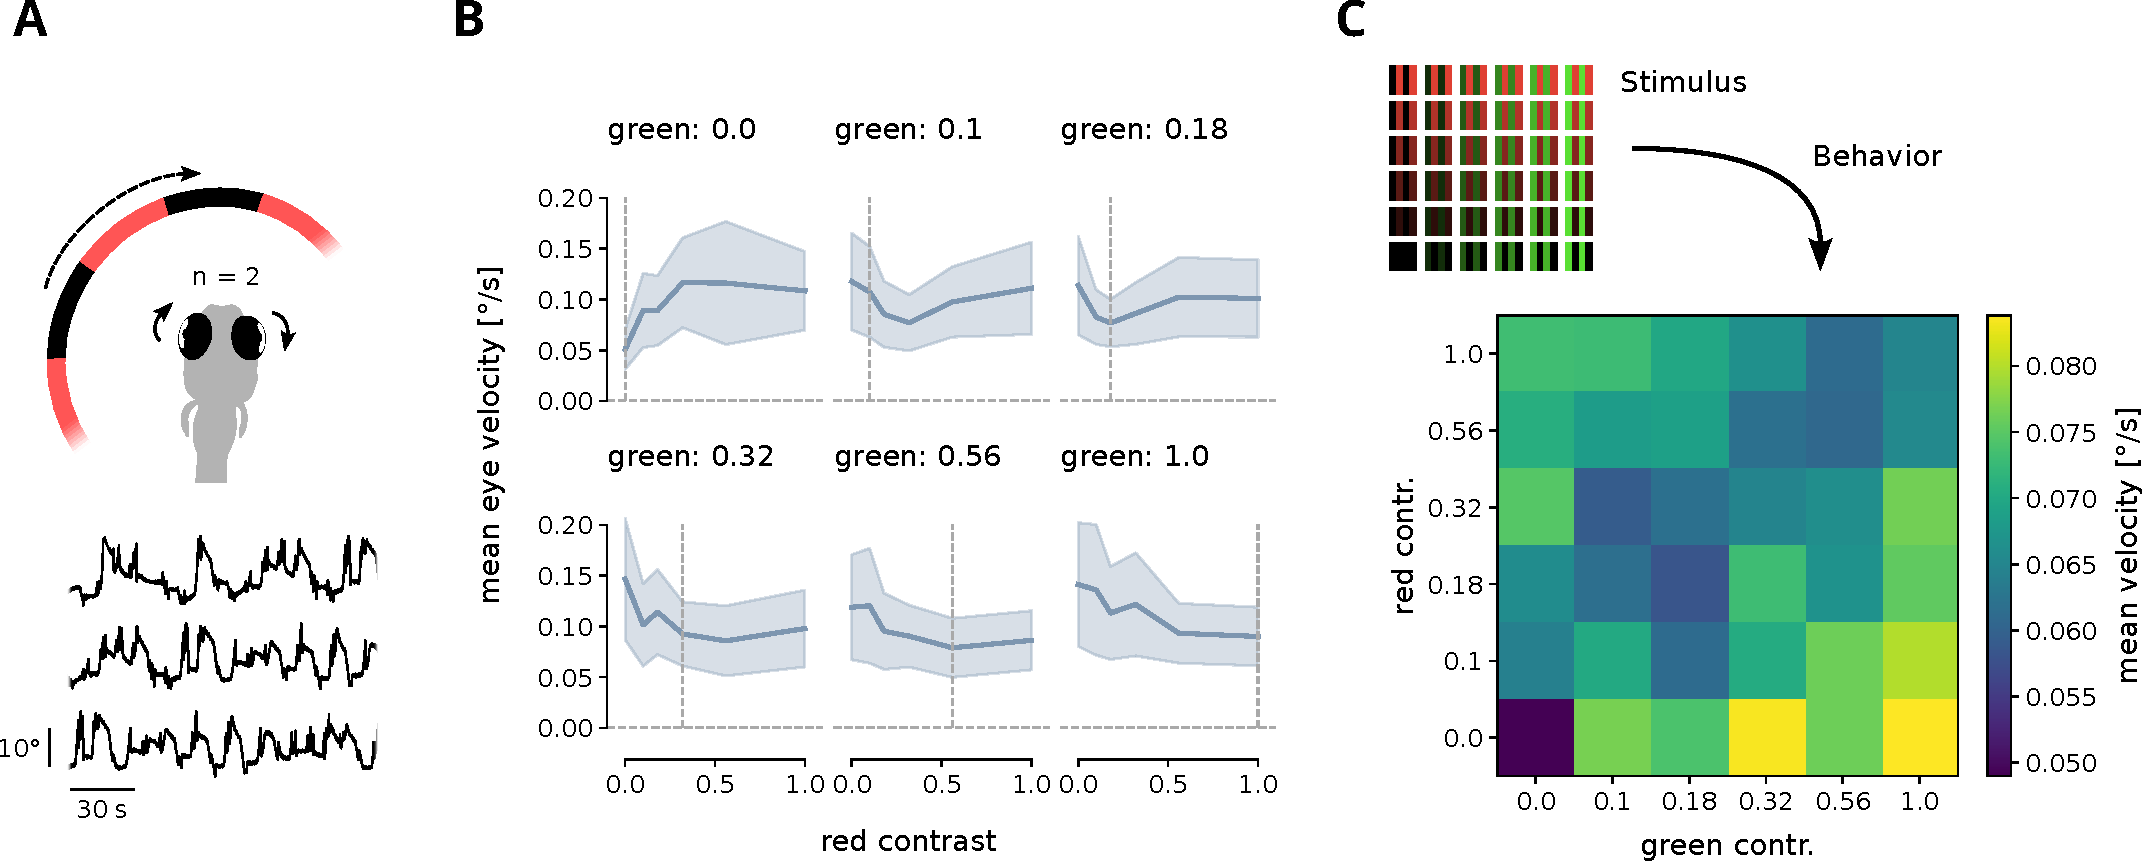
\includegraphics[width=\linewidth]{figures/contrast_curves_behav_test.pdf}
    \mycaption{Behavioral responses to different contrast levels.}{(A) Illustration of stimulus presentation and saccadic measurements to quantify the optokinetic response. (B) Mean and standard deviation of eye velocity for every level of green contrast (each subplot) as a function of all possible corresponding red contrast levels. The dashed vertical line illustrates the point in which, given that contrasts are perceived equally, only chromatic contrast should govern the behavioral response. If fish did not respond to exclusively color contrasts, the trough of the mean line should follow this point on the x-axis. (C) Stimulus and behavioral results quantified in the mean eye velocity are plotted in the same way as described in figure \ref{fig:calciumdata}. If the chromatic contrast did not contribute to the behavioral response, we would expect a diagonal of decreased eye velocity.}
    \label{fig:behavdata}
\end{figure}

\pagebreak
\section{Discussion}
  \label{chap:discussion}
  Our preprocessing pipeline successfully separated the direction-selective units from the population in the optic tectum. All units we analyzed were only active in their respective assigned motion direction despite the relatively low threshold we used to select them. These direction selective cells showed the lowest activity to isoluminant chromatic contrasts. The eye velocities also show this decrease, albeit not as strong as the cellular response.

\subsection{Direction selective cells in the optic tectum may be colorblind}

We found a decreased response, both on the level of the calcium activity of direction-selective tectal units - and behavior when the stimulus shifted from achromatic motion cues towards chromatic motion cues. This suggests that chromatic information is used less or not at all to encode motion direction in the optic tectum. 
% This can be compared to one of the notions of primates, where both pathways are separate \parencite{margaret1988segregationcolormovement}. 
The lack of a true zero cline and the fact that the response on the diagonal still increases with increasing chromatic contrast between the stripes can be interpreted in two different ways regarding the implementation of the current version of this experiment. The first interpretation could be, that there is in fact a true zero cline on the diagonal, but the stimulus levels we used were not diverse enough to target this region. If the stimulus is never truly isoluminant, a small amount of luminance contrast would still be able to stimulate the units. This luminance contrast would not increase with the intensity of both channels, however, the overall contrast sensitivity of the visual system is dependent on light intensity. This would also explain why the response to (seemingly) isoluminant chromatic contrasts increases, as the (not purely) chromatic contrasts increase. To test this hypothesis, a stimulation setup with increased precision in its tunability would be needed. In addition to that, one would need to increase the levels of contrasts that are presented. However, since all possible combinations of contrasts are presented, the number of stimulus phases needed would increase quadratically, making this approach less realistic. The second interpretation could be, that luminance may be the primary cue that is used for motion processing, but the optic tectum receives integrated information from the retina, which contains some color information. To our knowledge, there is no data on the processed color information in the optic tectum, only for direction-selective retinal ganglion cells \parencite{wangParallelChannelsMotion2020, ROBLES20142085}. 

\vspace{\baselineskip}

If we would compare these results to primates, we identify that fish only uses the first order of motion recognition. This first order relies solely on luminance and not color, indicating color blindness if we would stimulate with an isoluminant stimulus \parencite{orgerChannelingRedGreen2005, zhong1999isoluminant}. This is presented in our experiment. 

\vspace{\baselineskip}

For further studies, one could use color gratings moving in more directions than only the horizontal plane. For the zebrafish were three subtypes of direction-selective cells identified that can be used for a more robust dataset \parencite{nikolaou2012parametric}. Another suggestion can be the combination of color gratings in an optic flow stimulus, to have more natural stimuli. 

% \begin{itemize}
% %    \item -- Successfully filtered direction-selective units (see fig \ref{fig:heatmap})
% %    \item  -- we can see a degrading in signal to a  stimulus that only depends on the chromaticity of our color grating 
%     % \item this connection is not strong maybe because of the stimulus problem and the green contrast is brighter than the red contrast
%     % \item Problem of the z-score and how to achieve a true zero, pause duration 
%     % \item Problem of the pause duration in combination with the time it takes for fluorescence to stop (tied to the z-score issue).
%     % \item Problem of uncalibrated stimuli, but we still had stimuli with a local minimum so sufficient for this pilot study
%     % \item No clear zero-cline across the diagonal of the heatmaps could mean two things
%     % \begin{itemize}
%     %   %  \item There is a local minimum of activity which would go to 0 if the stimuli were calibrated and the contrast levels covered this occasion
%     %     \item Even with calibrated stimuli and a fine resolution of different contrast levels the diagonal would not be zero because some color information is included in the motion processing stream that passes through the optic tectum, resulting in a perception of motion that is then reflected behaviorally.
%     % \end{itemize}
%     %\item Problem with z-drift, maybe a higher concentration of agarose
%     \item confirming the results of the behavioral data from \cite{orgerChannelingRedGreen2005}
%     \item is different to what's going on in humans, % muss man noch genauer machen in der einleitung 
%     \item Problem of only two motion directions, which reduces the usable number of cells. The stimulus could move also down and up and all possible combinations.   \glqq The tuning properties of retinal ganglion cells have generally been determined using calcium imaging in their axon terminals outside the retina. Among direction-selective ganglion cells, three preferred directions are evident (Nikolaou et al. 2012, Gabriel et al. 2012, Lowe et al. 2013).\grqq{} \parencite{bollmannZebrafishVisualSystem2019}
%     \item 
    
% \end{itemize}


\subsection{Behaviour results were not as strong as the calcium data}

As for the decreased response in the data from the calcium imaging, in the behavioral response, we can estimate a shift to no motion for chromatic cues. In general, the response in the behavior analysis is weaker than in the calcium data, because the zero cline is not as strongly color coded as the one in the calcium imaging. That the behavioral readout is not completely in line with our calcium data and the previous studies \parencite{orgerChannelingRedGreen2005}, can be explained by the stimulus setup. The setup is optimized for our used calcium indicator and has 4 seconds of moving stimuli and 4 seconds of stationary stimulus with one specific color grating. To improve the behavioral readout one could introduce a gap of a given time so that the eye movements of the fish do not interfere with the next presented stimuli. 

\vspace{\baselineskip}

The main factor that explains elevated eye velocities, even for invisible stimuli, is our analysis pipeline. Since eye velocities are give in degrees per second, one of the stimuli will always result in negative velocities. To deal with this, we took the absolute velocities of both signals. The result is, that noise in the velocity signal that jitters around zero, and hence has a mean of approximately 0, becomes positive, with a mean above zero. To improve on this, a future iteration of our analysis pipeline should simply switch the sign of the signal dependent on the motion direction of the stimulus. This would keep the mean of noisy data around 0, while still making the velocities across the stimulus categories comparable.

\vspace{\baselineskip}

In contrast to \cite{orgerChannelingRedGreen2005}, who used the OMR (optomotor response) we used the OKR (optokinetic response), which can make a difference in response to an isoluminant stimulus. Against this hypothesis that OMR and OKR are different in the encoding of chromaticity is the argument that both share components in the pretectum and both encode similar large-field motion stimuli \parencite{wang2019selective, bollmannZebrafishVisualSystem2019}.


% \begin{itemize}
%     \item behavior data showed also no clear zero-cline, maybe there was still motion, therefore not all direction cells in the optic tectum are responsible for the behavior 
%     \item optomotor response is pretectum and optokinetic is tectum?
%     \item not the absolute but flip the signal in one direction 
% \end{itemize}


\subsection{Summary}
In conclusion, we found an indication that motion and color are processed separately in the zebrafish optic tectum and that the motion processing pathway only includes achromatic information. For the first time, we show that this may already be the case in the optic tectum. Additionally, we see the same pattern manifested in the behavioral output. 


\pagebreak
\printbibliography 

\pagebreak 
    \section{Appendix}
    \subsection{Experimental setup}

\begin{figure}[H]
    \centering
    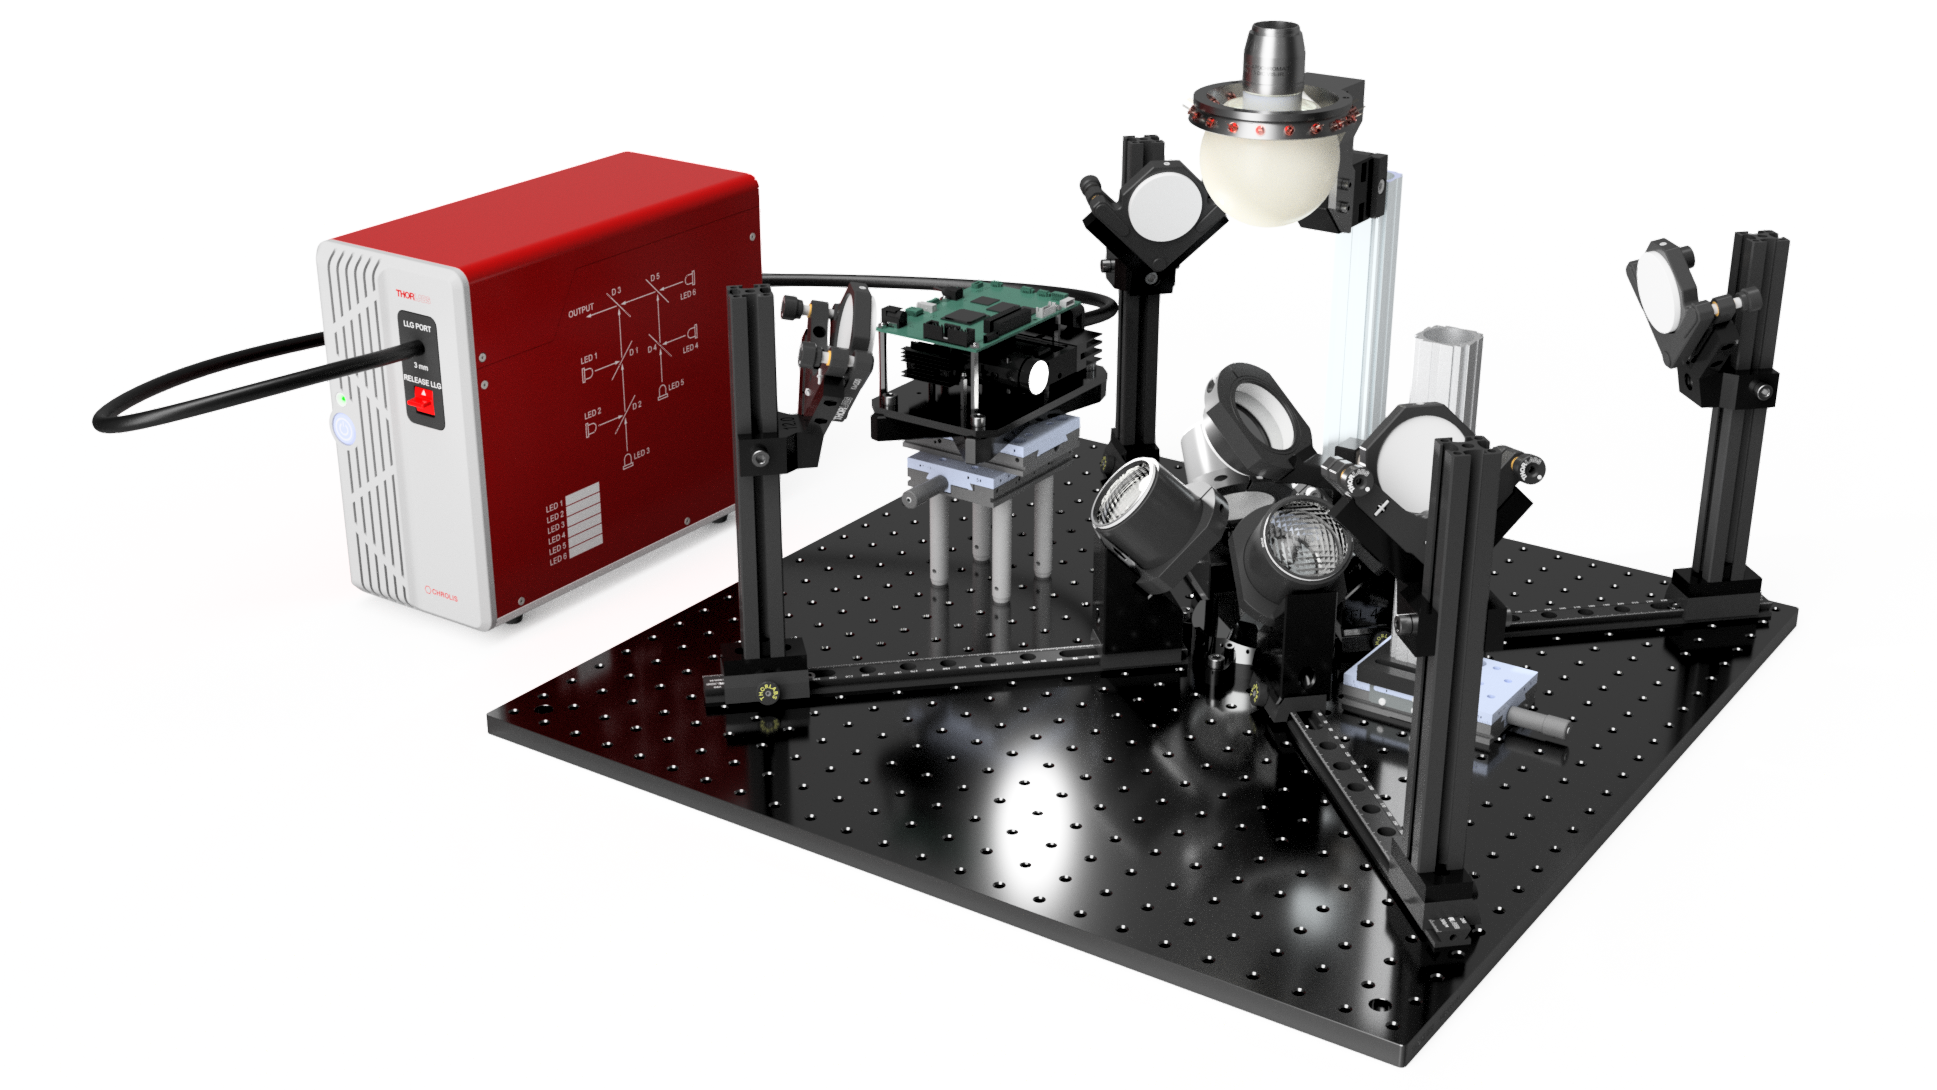
\includegraphics[width=\linewidth]{figures/Setup_CAD.png}
    \mycaption{Experimental setup.}{}
    \label{fig:setup}
\end{figure}


%\pagebreak
%\section{Appendix}
%  \label{chap:appendix}
%  \input{chapters/appendix.tex}

% Append pdf outputs from other programs to the document
% \includepdf[pages=-]{appendix/ab.pdf}
% \includepdf[pages=-]{appendix/cd.pdf}
% \includepdf[pages=-]{appendix/ef.pdf}

\end{document}